\documentclass{article}

\usepackage{float}
\usepackage{listings}
\usepackage{amsmath}
\usepackage[hidelinks]{hyperref} 	% per nascondere le box intorno alle voci dell'indice
\usepackage{graphicx}
\usepackage{subfiles}
% \usepackage[margin=1.5in]{geometry} % per diminuire il margine a bordo pagina
\usepackage[bottom]{footmisc} 		% per mettere il footnote a pie' di pagina
\usepackage[affil-it]{authblk}
\usepackage{listings}

\lstset{
  frame=bt,
  %frameround=tttt,
 %mathescape=true,
   language=Prolog,
   breaklines=true,
   showstringspaces=false,
   columns=flexible,
   numbers=none,
   %commentstyle=\color{MidnightBlue},
  %stringstyle=\color{gray},
   %stringstyle=\color{purple},
   basicstyle=\footnotesize\ttfamily,
   %literate=*{\$}{{\textcolor{arsenic}{\$}}}{1},
   tabsize=4
 }

% \bibliographystyle{plain}
% \usepackage{natbib}

% \hypersetup{
%     colorlinks=false, %set true if you want colored links
%     linktoc=all,     %set to all if you want both sections and subsections linked
%     linkcolor=blue,  %choose some color if you want links to stand out
% }

\setlength{\parindent}{0in}
\newcommand{\floor}[1]{\left\lfloor #1 \right\rfloor}
\newcommand{\ceil}[1]{\left\lceil #1 \right\rceil}

\date{}

% \renewcommand*\contentsname{Indice}

\begin{document}

\begin{titlepage}
  % \vspace*{\stretch{1.0}}
  \begin{center}
     \Large\textsc{Artificial Intelligence course\\University of Parma - A.Y. 2020/2021}\\
     \vspace{1cm}
     \Large\textbf{Skyscrapers in Prolog}\\
     \vspace{1cm}
     
      \large{\textsc{Author}: \texttt{Francesco Vetere}\\ \small \textsc{e-mail:} \href{mailto:francesco.vetere@studenti.unipr.it}{\texttt{francesco.vetere@studenti.unipr.it}} }
  \end{center}
  \vspace*{\stretch{2.0}}
\end{titlepage}

\pagebreak

% \tableofcontents

\section{Logic Programming}
Logic programming is a declarative programming paradigm: being declarative means that, generally speaking, the programmer provides the properties that the desired solution should have, rather than specifying the actual sequence of operations needed in order to obtain that solution (i.e.: imperative paradigm).\\

In particular, logic programming is based on formal logic: basically, any program is composed by
a list of facts and rules.\\
Given a certain goal, the idea is to demonstrate the truth of the goal using the knowledge base formed by facts and rules.\\

A key concept in logic programming is the one of unification.\\

In logic, unification is the algorithmic procedure used in solving equations involving symbolic expressions.\\
In other words, by replacing certain sub-expression variables with other expressions, unification tries to identify two symbolic expressions.\\

We say that two terms unify if they are the same term or if they contain variables that can be uniformly instantiated with terms in such a way that the resulting terms are equal.\\

In Prolog for example, when we try to unify two terms, the interpreter performs all the necessary variable instantiations, so that the terms really are equal afterwards: if the unification succeeds, Prolog also gives us the value of the instantiated variables.\\

\pagebreak

\section{Prolog}
Prolog is a logic programming language associated with artificial intelligence and computational linguistics, that has its roots in first-order logic, a formal logic, and uses a declarative style.\\

The language was implemented in the 70s by Alain Colmerauer, and since then it's been widely used for theorem proving, expert systems, automated planning and so on.\\

A Prolog program is generally composed by:\\
\begin{itemize}
  \item Facts (absolute truths about the domain)
  \begin{verbatim}
  father(a, b).
  \end{verbatim}
  \item Rules
  \begin{verbatim}
  grandfather(X, Y) :- father(X, Z), father(Z, Y).
  \end{verbatim}
\end{itemize}

Once the program has been written, we can ask the Prolog interpreter to solve a particular query.\\

In order to satisfy the goal, the backward chaining mechanism it's used:\\

If a fact that matches the query is known, the goal is satisfied;\\
Otherwise, for each rule whose consequences meet the question, the interpeter tries to test if each rule premise satisfies the query.\\

\pagebreak

Let's see a basic example of Prolog program.\\

\begin{lstlisting}
  %%%%%%%%%%%%%
  %%% Facts %%%
  %%%%%%%%%%%%%

  % Fact 1
  father(a, b).

  % Fact 2
  father(b, c).
  

  %%%%%%%%%%%%%
  %%% Rules %%%
  %%%%%%%%%%%%%

  % Rule 1
  % brother(X, Y) ==> true if X and Y have the same father, and X is not Y

  brother(X, Y) :- father(Z, X), father(Z, Y), X \= Y. 

  % Rule 2
  % grandfather(X, Y) ==> true if X is father of a generic Z, and that Z is father of Y

  grandfather(X, Y) :- father(X, Z), father(Z, Y).

\end{lstlisting}

Once the program has been loaded, we can ask for some queries to be solved.\\

\begin{lstlisting}
  ?- grandfather (a, c).
  true.
  
  ?- grandfather (X, c).
  X = a.

\end{lstlisting}

\pagebreak

\section{Skyscrapers puzzle}
The goal of this project is to implement the classic Skyscrapers puzzle using Prolog.\\

Skyscrapers is a game in which a matrix is given, and one should tell if that matrix is compliant or not according to some rules:\\

\begin{itemize}
  \item The numbers inside the matrix represent the heights of buildings.
  \item The numbers along the sides tell you how many skyscrapers a person standing in that spot can see.
  \item Each row and column contains each number only once.
\end{itemize}

Here are a few examples of how the clues help us to see which skyscrapers we might be able to see:\\

\begin{figure}[H]
  \centering
  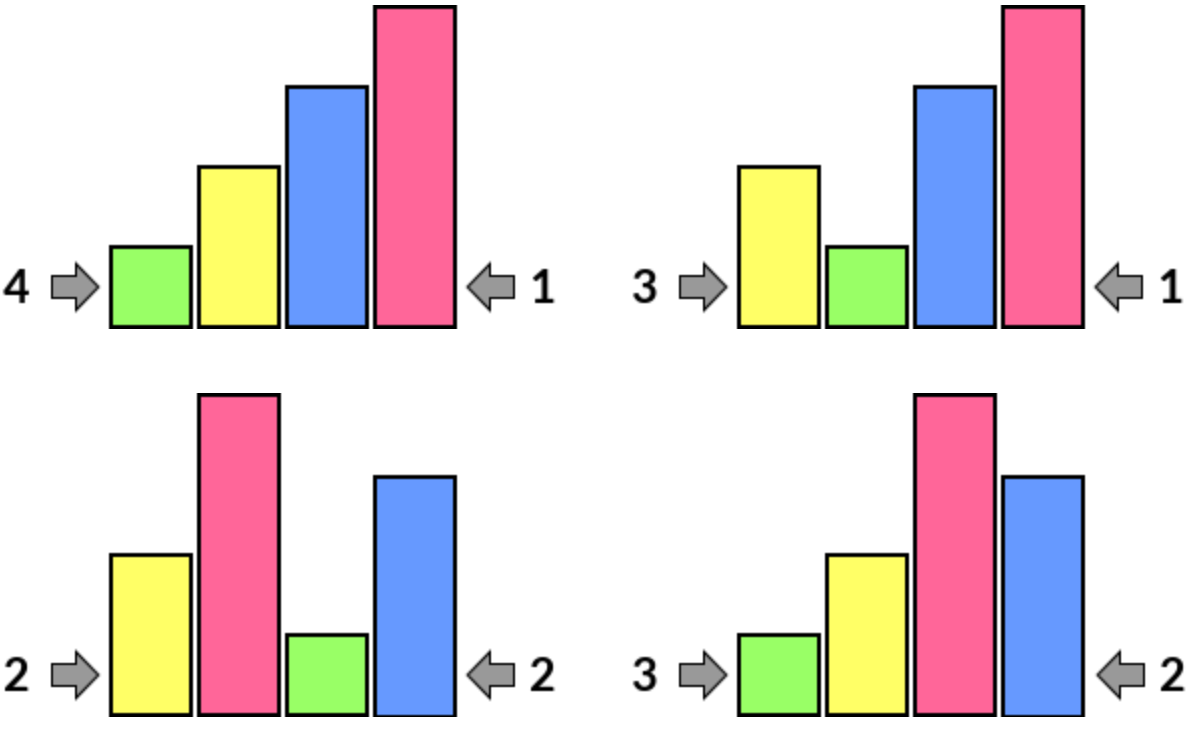
\includegraphics[scale=0.6]{img/skyscrapers-example.png}
  \caption{Skyscrapers example}
\end{figure}

\pagebreak

So, for example, this matrix is compliant with the rules of the game:\\

\begin{figure}[H]
  \centering
  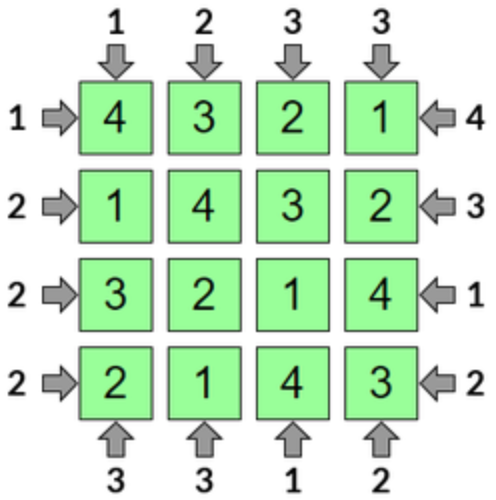
\includegraphics[scale=0.6]{img/skyscrapers-compliant.png}
  \caption{Skyscrapers compliant example}
\end{figure}

In order to represent a matrix in a \texttt{.txt} file, this particular format has been chosen:\\

\begin{verbatim}
  <N>
  <M[0,0]> ... <M[0,N-1]>
  ...
  <M[N-1,0]> ... <M[N-1,N-1]>
\end{verbatim}

So, for example, the following file \texttt{3x3.txt} represents a compliant matrix:\\

\begin{verbatim}
  5
  0 0 0 0 0
  0 1 2 3 1
  0 3 1 2 0
  2 2 3 1 0
  0 0 0 3 0
\end{verbatim}

(Note: 0's on the border are ignored)\\

\pagebreak

\section{Implementation}
In order to implement the puzzle in Prolog, a program \texttt{skyscrapers.pl} has been written.\\
It contains some basic predicates on lists and matrices, as well as some other predicates specific of the problem.\\

\begin{lstlisting}
  %%%%%%%%%%%%%%%%%%%%%%%%%%%%%%%%%%%%%%%%%%%%%%%%%%%%%%%%%%%%%%
  %%%%%%%%%%%%%%%%%%%%%%%%%%%%%%%%%%%%%%%%%%%%%%%%%%%%%%%%%%%%%%
  %%%%%%%%%%%%%%% Predicati di utilita' su liste %%%%%%%%%%%%%%%
  %%%%%%%%%%%%%%%%%%%%%%%%%%%%%%%%%%%%%%%%%%%%%%%%%%%%%%%%%%%%%%
  %%%%%%%%%%%%%%%%%%%%%%%%%%%%%%%%%%%%%%%%%%%%%%%%%%%%%%%%%%%%%%
  
  
  % member(elem, L) ==> true se L contiene elem
  member(X, [X | _]).
  member(X, [_ | T]) :- member(X, T).
  
  % append(L, R, RIS) ==> RIS è la lista L concatenata con R
  append([], R, R).
  append([H | T], R, [H | TEMP]) :- append(T, R, TEMP).
  
  % reverse(A, B) ==> B è la lista A rovesciata
  reverse([], []).
  reverse([H | T], RIS) :- reverse(T, TEMP), append(TEMP, [H], RIS).
  
  % length(A, LEN) ==> LEN è pari alla lunghezza della lista A
  len([], 0).
  len([_ | T], RIS) :- len(T, TEMP), RIS is TEMP + 1.
  
  % removeFirstLast(A, RIS) ==> RIS è la lista A privata del primo e dell'ultimo elemento
  removeFirstLast(L, RIS) :- removeFirst(L, TEMP), removeLast(TEMP, RIS).
  
  % removeFirst(A, RIS) ==> RIS è la lista A privata del primo elemento
  removeFirst([], []).
  removeFirst([_], []).
  removeFirst([_ | T], T). 
  
  % removeLast(A, RIS) ==> RIS è la lista A privata dell'ultimo elemento
  removeLast([], []).
  removeLast([_], []).
  removeLast(X, Y) :- reverse(X, [_ | T]), reverse(T, Y).
  
  % unique(L) ==> true se L contiene valori unici
  unique([]).
  unique([H | T]) :- \+ member(H, T), unique(T).
  
  % uniqueFirstLast(L) ==> true se L, privata del primo e ultimo elemento (quelli di bordo!) contiene valori unici
  uniqueFirstLast(L) :- removeFirstLast(L, LNew), unique(LNew).
  
  


  %%%%%%%%%%%%%%%%%%%%%%%%%%%%%%%%%%%%%%%%%%%%%%%%%%%%%%%%%%%%%%
  %%%%%%%%%%%%%%%%%%%%%%%%%%%%%%%%%%%%%%%%%%%%%%%%%%%%%%%%%%%%%%
  %%%%%%%%%%%%%% Predicati di utilita' su matrici %%%%%%%%%%%%%%
  %%%%%%%%%%%%%%%%%%%%%%%%%%%%%%%%%%%%%%%%%%%%%%%%%%%%%%%%%%%%%%
  %%%%%%%%%%%%%%%%%%%%%%%%%%%%%%%%%%%%%%%%%%%%%%%%%%%%%%%%%%%%%%
  
  
  % uniqueMatrixFirstLast(M) ==> true se la matrice M contiene liste uniche, private del primo e ultimo elemento (quelli di bordo!)
  uniqueMatrixFirstLast([]).
  uniqueMatrixFirstLast([H | T]) :- 
      uniqueFirstLast(H), uniqueMatrixFirstLast(T).
  
  % isMatrixSquare(M) ==> true se M è almeno 2x2 ed è quadrata
  isMatrixSquare([H | T]) :- len(H, COLS), len([H | T], ROWS), 
                             ROWS >= 2, COLS >= 2, ROWS == COLS.
  
  % transposeMatrix(M, MT) ==> MT contiene la trasposta di M
  transposeMatrix([[] | _], []).
  transposeMatrix(Matrix, [FirstColumn | TransposedRestMatrix]) :- 
      splitMatrix(Matrix, FirstColumn, RestMatrix), % FirstColumn diventa la prima riga nella matrice trasposta
      transposeMatrix(RestMatrix, TransposedRestMatrix).
  
  % splitMatrix(Matrix, FirstColumn, RestOfMatrix) ==> Matrix viene divisa in FirstColumn e RestOfMatrix
  splitMatrix([], [], []).
  splitMatrix(
      [[FirstEl | RestFirstRow] | OtherRows],   							% Matrix
      [FirstEl | RestFirstCol],  														 	% First column
      [RestFirstRow | RestOtherRows]												 	% Rest of the matrix
  ) :- splitMatrix(OtherRows, RestFirstCol, RestOtherRows).
  
  
  %%%%%%%%%%%%%%%%%%%%%%%%%%%%%%%%%%%%%%%%%%%%%%%%%%%%%%%%%%%%%%%%%%%%%%%%%%%%%%
  %%%%%%%%%%%%%%%%%%%%%%%%%%%%%%%%%%%%%%%%%%%%%%%%%%%%%%%%%%%%%%%%%%%%%%%%%%%%%%
  %%%%%%%%%%%%%%%%%%%% Predicati specifici di skyscrapers %%%%%%%%%%%%%%%%%%%%%%
  %%%%%%%%%%%%%%%%%%%%%%%%%%%%%%%%%%%%%%%%%%%%%%%%%%%%%%%%%%%%%%%%%%%%%%%%%%%%%%
  %%%%%%%%%%%%%%%%%%%%%%%%%%%%%%%%%%%%%%%%%%%%%%%%%%%%%%%%%%%%%%%%%%%%%%%%%%%%%%
  
  
  % countChangesMax(L, RIS) ==> RIS è pari al numero di volte in cui il massimo cambia nella lista L (da sinistra a destra) 
  countChangesMax([0 | T], RIS) :- countChangesMaxAux(T, 0, 1, RIS).
  countChangesMax(L, RIS) :- countChangesMaxAux(L, 0, 0, RIS).
  
  % countChangesMaxAux(L, RIS) ==> RIS è pari al numero di volte in cui il massimo cambia nella lista L (da sinistra a destra)
  % 															 con massimo corrente pari a CurrentMax e accumulatore Acc
  countChangesMaxAux([H | T], CurrentMax, Acc, RIS) :-
      H > CurrentMax,
      AccNew is Acc + 1,
      countChangesMaxAux(T, H, AccNew, RIS).
   
  countChangesMaxAux([H | T], CurrentMax, Acc, RIS) :-
      H =< CurrentMax,
      countChangesMaxAux(T, CurrentMax, Acc, RIS).
   
  countChangesMaxAux([], _, Acc, Acc).
  
  % isListCompliant(L) ==> true se la lista L rispetta il vincolo del gioco skyscrapers previsto per ogni riga/colonna:
  % 											 il primo elemento della lista deve essere uguale al numero di massimi incontrati
  % 											 lungo il resto della lista
  isListCompliant([0 | _]). 
  isListCompliant([H | T]) :-  countChangesMax(T, MAXS), H == MAXS. 
  
  % checkRuleForward(M) ==> true se la matrice M rispetta il vincolo del gioco skyscrapers per ogni riga, da sx a dx
  checkRuleForward([]).
  checkRuleForward([H | T]) :-
      isListCompliant(H), checkRuleForward(T).
  
  % checkRuleBackward(M) ==> true se la matrice M rispetta il vincolo del gioco skyscrapers per ogni riga, da dx a sx
  checkRuleBackward([]).
  checkRuleBackward([H | T]) :-
      reverse(H, HReverse), isListCompliant(HReverse), checkRuleBackward(T).
  
  % isMatrixCompliant(L) ==> true se la matrice M rispetta le regole del gioco skyscrapers
  isMatrixCompliant(M) :-
      isMatrixSquare(M), 																				% controllo che la matrice sia quadrata
  
      removeFirstLast(M, M1), uniqueMatrixFirstLast(M1),        % controllo che all'interno dei bordi vi siano valori unici:
                                                                % elimino prima e ultima riga, e controllo se le restanti righe
                                                                % contengono valori unici a meno di prima e ultima colonna
  
      checkRuleForward(M),																			% controllo la regola da sx a dx
      checkRuleBackward(M),																			% controllo la regola da dx a sx
  
      transposeMatrix(M, MT),
  
      checkRuleForward(MT),																			% traspongo e controllo la regola da sx a dx
      checkRuleBackward(MT).																		% traspongo e controllo la regola da dx a sx
  
  

  %%%%%%%%%%%%%%%%%%%%%%%%%%%%%%%%%%%%%%%%%%%%%%%%%%%%%%%%%%%%%%
  %%%%%%%%%%%%%%%%%%%%%%%%%%%%%%%%%%%%%%%%%%%%%%%%%%%%%%%%%%%%%%
  %%%%%%%%%%%%%%% Lettura della matrice da file %%%%%%%%%%%%%%%%
  %%%%%%%%%%%%%%%%%%%%%%%%%%%%%%%%%%%%%%%%%%%%%%%%%%%%%%%%%%%%%%
  %%%%%%%%%%%%%%%%%%%%%%%%%%%%%%%%%%%%%%%%%%%%%%%%%%%%%%%%%%%%%%
  
  
  % leggi_lista_str(L, F) ==> L è la lista letta dal file F
  leggi_lista_str(L, F):- see(F), leggi_lista_str(L), seen.
  leggi_lista_str([S|R]):- leggi_atomo(S), S\==end_of_file, !, leggi_lista_str(R).
  leggi_lista_str([]).
  leggi_atomo(end_of_file):- at_end_of_stream, !.
  leggi_atomo(S):- leggi_lista_car(L), name(S, L).
  leggi_lista_car([C|R]):- get0(C), C\==10, C\==32, C\==(-1), !, leggi_lista_car(R).
  leggi_lista_car([]).
  
  % list_to_matrix(List, N, Matrix) ==> Matrix è la matrice N x N costruita a partire da List
  list_to_matrix([], _, []).
  list_to_matrix(List, Size, [Row|Matrix]):-
      list_to_matrix_row(List, Size, Row, Tail),
      list_to_matrix(Tail, Size, Matrix).
  
  list_to_matrix_row(Tail, 0, [], Tail).
  list_to_matrix_row([Item|List], Size, [Item|Row], Tail):-
      NSize is Size-1,
      list_to_matrix_row(List, NSize, Row, Tail).
  
  % build_matrix(File, Matrix) ==> Matrix è la matrice letta dal file File
  build_matrix(File, Matrix) :- leggi_lista_str([H | T], File), list_to_matrix(T, H, Matrix).
  
  
  %%%%%%%%%%%%%%%%%%%%%%%%%%%%%%%%%%%%%%%%%%%%%%%%%%%%%%%%%%%%%%
  %%%%%%%%%%%%%%%%%%%%%%%%%%%%%%%%%%%%%%%%%%%%%%%%%%%%%%%%%%%%%%
  %%%%%%%%%%%%%%%%%%% Predicato principale %%%%%%%%%%%%%%%%%%%%%
  %%%%%%%%%%%%%%%%%%%%%%%%%%%%%%%%%%%%%%%%%%%%%%%%%%%%%%%%%%%%%%
  %%%%%%%%%%%%%%%%%%%%%%%%%%%%%%%%%%%%%%%%%%%%%%%%%%%%%%%%%%%%%%
  
  
  % skyscrapers(File) ==> true se File contiene una matrice in accordo con le regole del gioco
  skyscrapers(File) :- build_matrix(File, Matrix), isMatrixCompliant(Matrix).
\end{lstlisting}

\pagebreak

Now, we can test our program giving in input some compliant matrices, and verifying that the main goal is satisfied.\\

\begin{verbatim}
> swipl

> ?- consult('skyscrapers.pl').

> ?- skyscrapers('matrices/3x3.txt').
  		==> true.

> ?- skyscrapers('matrices/4x4.txt').
  		==> true.

> ?- skyscrapers('matrices/5x5.txt').
  		==> true.

> ?- skyscrapers('matrices/6x6.txt').
   		==> true.
\end{verbatim}

\end{document}